\begin{recipe}{Pressure Cooker Buffalo Chicken}{4 Portions}{10 Minutes}

\ingredient[2]{lbs}{Chicken}
\ingredient[\fr{2}{3}]{Cup}{Frank's Red Hot}
\ingredient[\fr{1}{3}]{Cup}{Water}
\ingredient[1]{Tbsp}{Butter}
Put all ingredients into the pressure cooker.\\~\\~\\~\\~\\

\newstep
Once the pressure has built, cook for 4 additional minutes on medium.\\~\\

\newstep
Once cooking is finished, turn off the heat and allow the pressure cooker to cool until the pressure is released. Once cool, shred the chicken.

\end{recipe}

\begin{center}
~\\~\\
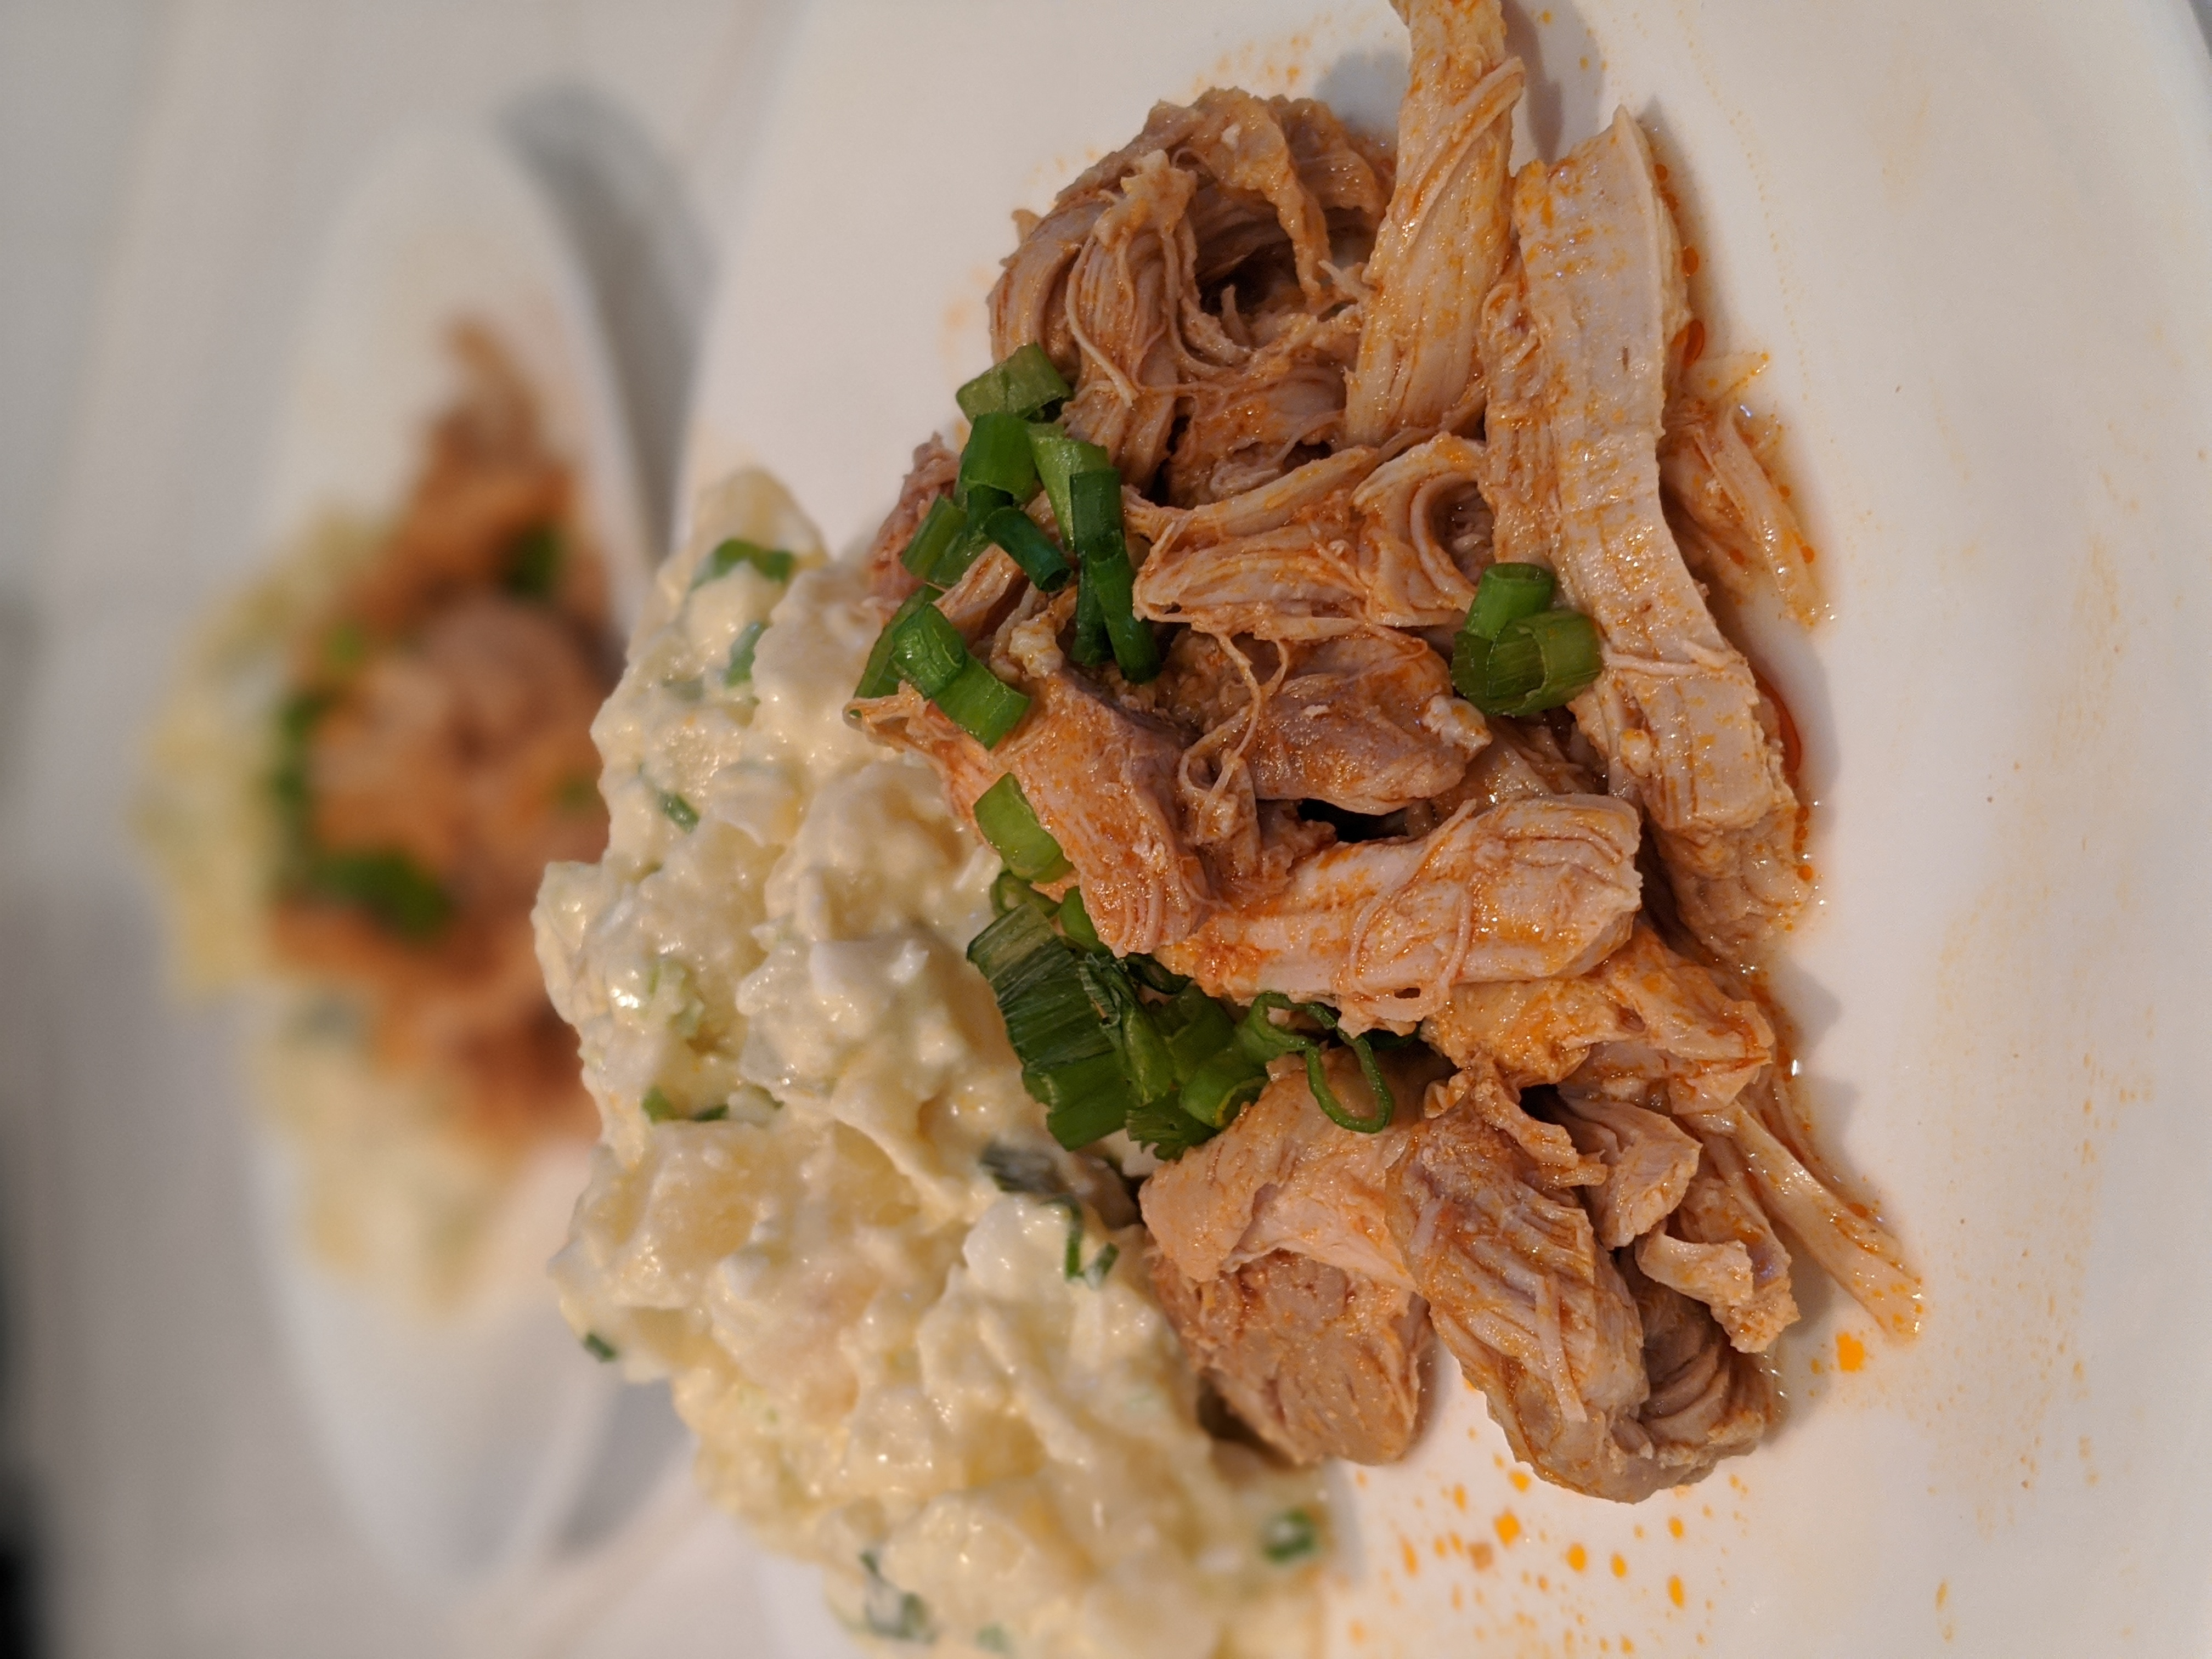
\includegraphics[width=4in,angle=270]{buffalo_chicken_pressure_cooker.jpg}
\end{center}